\documentclass[11pt, handout]{beamer}
\usepackage[utf8]{inputenc} 
\usepackage[T1]{fontenc}
\usepackage{lmodern}
\usepackage{graphicx}
\usepackage[french]{babel}
\usepackage{graphicx}
\usetheme{Rochester}
\definecolor{structcoul}{rgb}{0.82,0.2,0.2}
%%\setbeamercolor{structure}{fg=structcoul, bg=structcoul!40}
% \setbeamertemplate{footline}{
% \leavevmode%
% \hbox{\hspace*{-0.12cm}
% \begin{beamercolorbox}[wd=.802\paperwidth,ht=2.25ex,dp=1ex,center]{section in head/foot}%
% 	\usebeamerfont{section in head/foot}\insertshorttitle
% \end{beamercolorbox}%
% \begin{beamercolorbox}[wd=.21\paperwidth,ht=2.25ex,dp=1ex,right]{section in head/foot}%
% 	\usebeamerfont{section in head/foot}\insertshortdate{}\hspace*{1em}
% 	\insertframenumber{} / \inserttotalframenumber\hspace*{2ex}
% \end{beamercolorbox}}%
% }
\setbeamertemplate{caption}[numbered]
\setbeamertemplate{footline}
{
  \leavevmode%
  \hbox{%
  \begin{beamercolorbox}[wd=.40\paperwidth,ht=2.25ex,dp=1ex,center]{author in head/foot}%
    \usebeamerfont{author in head/foot}\insertauthor \
  \end{beamercolorbox}%
  \begin{beamercolorbox}[wd=.30\paperwidth,ht=2.25ex,dp=1ex,center]{title in head/foot}%
    \usebeamerfont{title in head/foot}\insertsection
  \end{beamercolorbox}%
  \begin{beamercolorbox}[wd=.30\paperwidth,ht=2.25ex,dp=1ex,right]{date in head/foot}%
    \usebeamerfont{date in head/foot}\insertshortdate{}\hspace*{2em}
    \insertframenumber{} / \inserttotalframenumber\hspace*{2ex} 
  \end{beamercolorbox}}%
  \vskip0pt%
}


\title[EadGen]{EadGen, un environnement ouvert de production en ligne basé sur 
XML et XSL-T}
%\subtitle{sous-titre}
\author{Julien Baron, Grégoire Gutzwiller, \\ Guillaume Minette de Saint-Martin}
\date[18/05/2015]{Lundi 18 Mai 2015}
\titlegraphic{
\includegraphics[scale=0.20]{resources/logoInsa.jpeg}}

\logo{
\includegraphics[scale=0.06]{resources/logoInsa.jpeg}}

\begin{document}
\begin{frame}[plain]
	\maketitle
\end{frame}

%%%%%%% LE SOMMAIRE
\author{Grégoire Gutzwiller}
\section*{Sommaire}
\begin{frame}
	\frametitle{Sommaire}
	\tableofcontents
\end{frame}

%%%%%%% CONTEXTE
\author{Guillaume Minette de Saint-Martin}
\section{Contexte et Objectifs}
\begin{frame}
	\frametitle{Introduction}
	\begin{block}{Pourquoi EadGen}
		\begin{itemize}
			\item Besoin de mettre en ligne les ressources pédagogiques 
			\item Plusieurs techniques existent
			\item Exigences de compétences informatique
		\end{itemize}
	\end{block}
\end{frame}

\author{Guillaume Minette de Saint-Martin}
\begin{frame}
	\frametitle{Méthodes existantes}
	\begin{block}{Production page par page}
		\begin{itemize}
			\item Très bons résultats
			\item Personnalisation possible à l'extrème
			\item Chronophage
			\item Peu maintenable
		\end{itemize}
	\end{block}
\end{frame}
\begin{frame}
	\frametitle{Méthodes existantes}
	\begin{block}{Pages dynamiques}
		\begin{itemize}
			\item Génération des pages automatisée
			\item Rapidité de production
			\item Maintenabilité accrue
			\item Peu de personnalisation
			\item Difficilement généralisable à différents domaines
		\end{itemize}
	\end{block}
\end{frame}
\begin{frame}
	\frametitle{Méthodes existantes}
	\begin{block}{Transformation de structure}
		\begin{itemize}
			\item Mélange entre production page par page et les pages dynamiques
			\item Utilisation de langages intermédiaires pour définir les données et les transformations
			\item Requière l'utilisation de langages intermédiaires 
			\item Lourd à l'écriture
		\end{itemize}
	\end{block}
\end{frame}

%%%%%%% ENVIRONNEMENT
\author{Julien Baron}
\section{L'environnement EadGen}
EadGen est utilisable en ligne par l'ensemble des personnes intervenant sur un document. De l'auteur au responsable de collection en passant par les graphistes et autres membres, la production doit rester accessible.

\subsection{Fondements de Eadgen}

Contrairement aux méthodes existantes, EadGen propose un langage auteur ouvert reposant sur XML. Ceci permet à chaque membre intervenant sur la chaine de production de paramétrer l'outil selon son expertise et ses besoins relatifs aux outils qu'il utilise.

La chaine de production repose essentiellement sur les spécifications établies entre les auteurs, qui fournissent la matière première pédagogique, et le responsable de collection. Ils vont établir ensemble le besoin de médiatisation du document.

EadGen permet ici via des pré-traitements d'éviter l'emploi trop lourd du XML grâce à son langage auteur ouvert comme l'on pourrait le faire en HTML.

\subsection{Production basée sur XSL-T}

Produire un document c'est convertir une structure source, la matière première pédagogique, en structure cible : le document produit où l'on mettra en avant l'organisation pédagogique et l'interaction.

L'automatisation de cette production implique de modéliser ces structures et spécifier leurs règles de transformation. De plus, pour une même collection, la structure cible aura toujours le même modèle, quelque soit le contenu de la source. C'est là qu'intervient le langage de transformation XSL-T.

\subsection{Architecture et Fonctionnement}

\paragraph{}
Ici, la chaine de production permet de simplifier la définition du langage auteur extensible et la production du HTML cible. Pour une collection donnée, le responsable va avec les auteurs retenir les concepts importants pour la médiatisation de leurs cours et créer un jeu de balises associé.

Ensuite, avec un graphiste, le responsable va définir l'action des balises sur la production finale toujours grâce à EadGen qui va convertir une maquette HTML en xsl-template qui permettra la traduction du XML source en HTML final.

Double avantage, l'auteur dispose d'un fort pouvoir d'expression grâce au balisage léger, puis ces balises sont converties par le compilateur en XML puis en HTML automatiquement.

\paragraph{}
Pour illustrer la puissance du langage ouvert EadGen, un exemple pour un cours de chimie est donné. L'enseignant souhaite appuyer la dangerosité de certains produits dans les cours et exercices interactifs. Il définit alors avec le responsable de collection une balise "\$tox" qui produira une alerte.

Après introduction de cette balise dans le vocabulaire du langage, l'auteur n'aura à définir qu'une seule fois : \texttt{\$tox chlore}, dans une de ses productions sources pour que l'alerte se retrouve dans chaque occurrence du mot "chlore" dans n'importe quel document cible. Cette alerte sera présentée de la manière retenue par le graphiste dans sa maquette au sein du document final via le processus présenté plus haut.

\paragraph{}
La puissance de EadGen repose donc dans la séparation du contenu et de la forme finale grâce au langage de balises léger et à la création simplifiée des transformations XSL-T à partir de maquettes. Cela permet de plus de prévenir les problèmes liés aux différents supports cibles, navigateurs ou imprimantes, en spécifiant plusieurs maquettes. La médiatisation peut donc être automatique et transcrire clairement les éléments de pédagogie de l'auteur.

%%%%%%% LANGAGES
\author{Grégoire Gutzwiller}
\section{Conception et traitement des langages}
\begin{frame}
	\frametitle{Forme générique du langage auteur}
	\framesubtitle{Le langage auteur : quel but ?}

	\begin{block}{Critères pour le langage auteur}
		\begin{itemize}
			\item Facile d'utilisation
			\item Extensible
			\item Fonctionnement par balises
		\end{itemize}
	\end{block}

	\begin{block}{Syntaxe d'une balise}
		\begin{itemize}
			\item Nom
			\item Champ de méta-données optionnel
			\item Paramètre principal optionnel
		\end{itemize}
	\end{block}
\end{frame}

\begin{frame}
	\frametitle{Forme générique du langage auteur}
	\framesubtitle{Les balises}

	\begin{block}{Portée d'une balise}
		L'effet de la balise perdure jusqu'à qu'elle rencontre
		une balise plus importante qu'elle.
	\end{block}

	\begin{block}{Forme d'une balise}
		\texttt{\$sonNom (ses méta-données) son paramètre principal}
	\end{block}
\end{frame}

\begin{frame}
	\frametitle{Spécification du vocabulaire}

	\begin{itemize}
		\item Définit le vocabulaire et la sémantique
		\item Est donné sous la forme de documents XML
	\end{itemize}

	\begin{block}{Exemple}
		<Balise
		\ \ \ \	nom = «tox» priorité = «50» \\
		\ \ \ \	concerne = «nom du produit concerne» \\
		\ \ \ \	porte = «consignes de sécurité associées» \\
		\ \ \ \	detecte\_occurrence= «bulle» \\
		\ \ \ \	cree\_bulle\_avec= «contenu» \\
		\ \ \ \	table\_associée = «Produits Toxiques» \\
		\ \ \ \	references\_croisée = «oui» \\
		\ \ \ \	nom\_xml= «prodtox» /> \\
	\end{block}
\end{frame}

\begin{frame}
	\frametitle{Fonctionnement interne d'EadGen}

	\begin{figure}
		\centering
		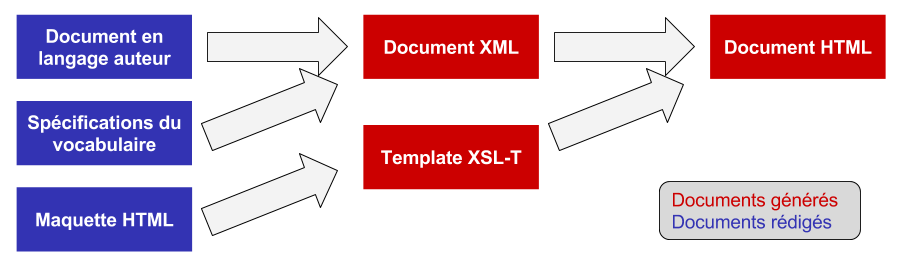
\includegraphics[scale=0.32]{resources/fctEadgen.png}
		\caption{Documents générés par EadGen}
	\end{figure}
\end{frame}



%%%%%%% DEMONSTRATION
\author{Julien Baron}
\section{Démonstration}

\begin{frame}
	\frametitle{Exemple de page EadGen}
	\begin{figure}
		\centering
		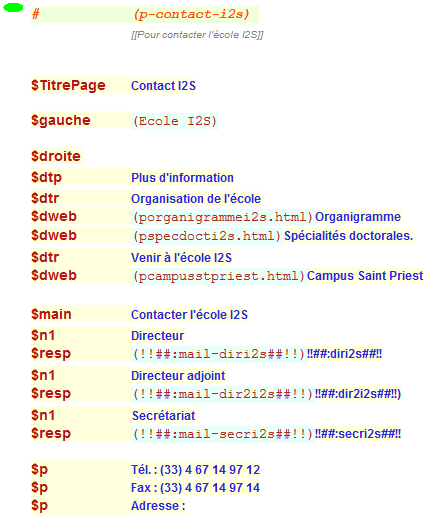
\includegraphics[scale=0.5]{resources/CaptureTemplateBeau.PNG}
	\end{figure}
	\end{frame}
\begin{frame}
	\frametitle{Fichier de définition de variables}
	\begin{figure}
		\centering
		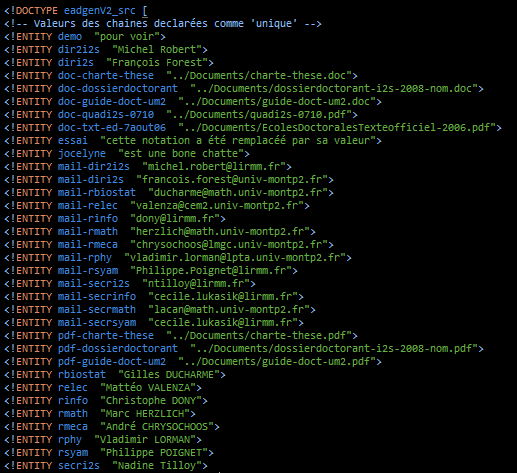
\includegraphics[scale=0.58]{resources/variables.PNG}
	\end{figure}
	\end{frame}
\begin{frame}
	\frametitle{Exemple de balise}
	\begin{figure}
		\centering
		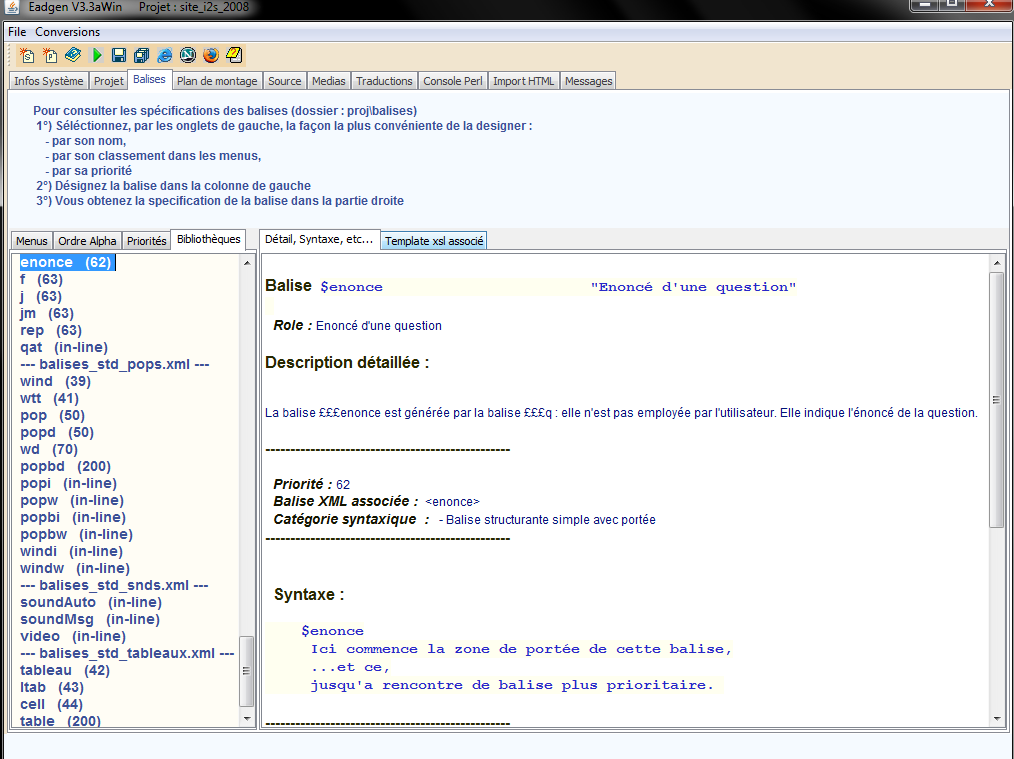
\includegraphics[scale=0.33]{resources/balise.PNG}
	\end{figure}
	\end{frame}
\begin{frame}
	\frametitle{Exécution de EadGen}
	\begin{figure}
		\centering
		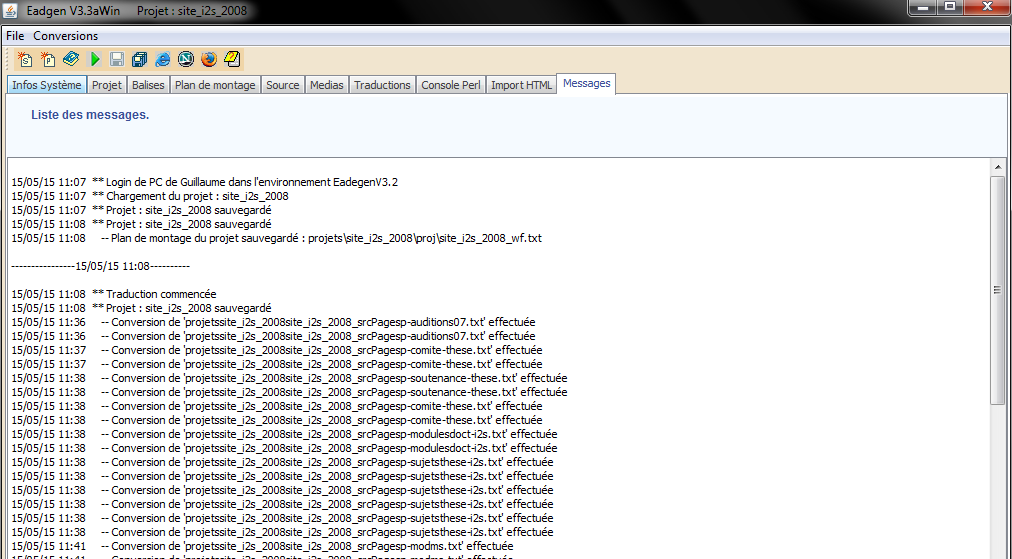
\includegraphics[scale=0.39]{resources/messages.PNG}
	\end{figure}
	\end{frame}
\begin{frame}
	\frametitle{Résultat}
	\begin{figure}
		\centering
		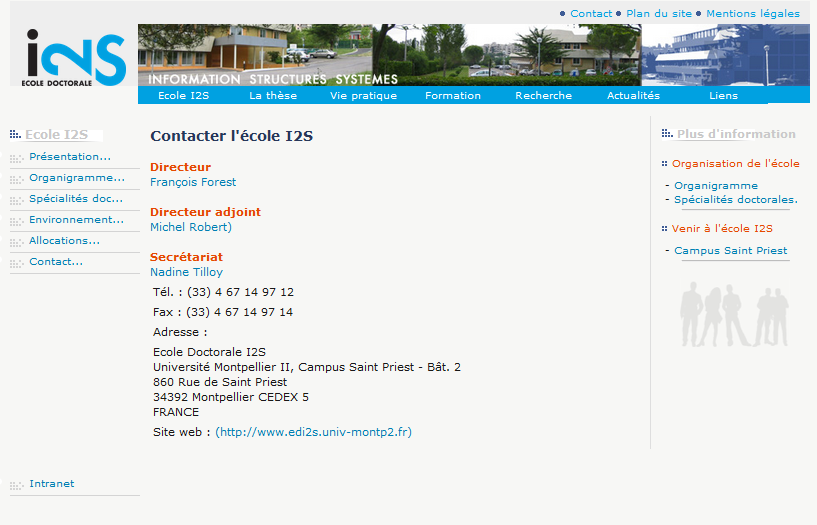
\includegraphics[scale=0.47]{resources/pageHttp.PNG}
	\end{figure}
	\end{frame}

\end{document}